\section{Impact of wide SRF wings}
%=================================
To minimise the amount of monochromatic transmittances calculations that are required, the wings of instrument SRFs are truncated. The frequency at which this truncation occurs is somewhat subjective and requires visual inspection of the SRF wings to determine if the data is real, noise, or an artifact of the measurement system. This section is a short description of how this truncation can affect the results when an SRF has wide wings.

Generally, the truncation frequency is selected when the response values decreases below a value of 10\superscript{-4}. In processing the NOAA-16 AVHRR/3 channel 3B data from the \href{http://www.star.nesdis.noaa.gov/smcd/spb/fwu/solar_cal/spec_resp_func}{NESDIS/STAR website}, it was noticed that the shortwave wing of the SRF extended almost two full widths at half-maximum (FWHM) (see the top panel of figure \ref{fig:avhrr3_n16.ch3b.srf}). Close inspection of this shortwave wing revealed that the data was quantised at the 10\superscript{-3} level, and that the wing had a constant value of 0.002 from approximately 2900-3300\invcm{} (see the bottom panel of figure \ref{fig:avhrr3_n16.ch3b.srf}). Because this value is larger than the nominal cutoff magnitude, the entire wing was included in the initial processing.

As shown in figure \ref{fig:avhrr3_n16.ch3b.srf}, frequencies were selected at which to truncate the SRF. The selected $f1$ and $f2$ cutoff frequencies for this channel were 2290\invcm{} and 2920\invcm{}. The impact of this truncation is shown in table \ref{tab:avhrr3_n16.ch3b.srf} where the effective temperatures for a blackbody temperature of 285K differ by 0.13K.

\begin{figure}[htp]
  \centering
  \includegraphics[bb=90 265 540 660,clip,scale=1]{graphics/long_baseline/avhrr3_n16.ch3B.srf.eps}
  \caption{NOAA-16 AVHRR/3 channel 3B SRF indicating the frequencies at which the original SRF data was truncated prior to interpolation. \textbf{(Top panel)} The entire SRF. \textbf{(Bottom panel)} A magnification showing the elevated wings of the SRF.}
  \label{fig:avhrr3_n16.ch3b.srf}
\end{figure}

\begin{table}[htp]
  \centering
  \begin{tabular}{l *{4}{r@{.}l}}
    \hline
                           & \multicolumn{2}{c}{\textbfm{T_{eff}}} & \multicolumn{2}{c}{\textbfm{\nu_o}} & \multicolumn{2}{c}{\textbfm{a_0}} & \multicolumn{2}{c}{\textbfm{a_1}} \\
    \rb{\textbf{SRF Type}} & \multicolumn{2}{c}{(K)}               & \multicolumn{2}{c}{(\invcm)}        & \multicolumn{2}{c}{(K)}           & \multicolumn{2}{c}{(K/K)} \\
    \hline\hline\vspace{-0.5em}\\
    Original (no cutoff)   &   286&25 & 2697&5630 & 2&268358 & 0&996416 \vspace{0.5em}\\ 
    Original (with cutoff) &   286&12 & 2696&4477 & 2&017304 & 0&996841 \vspace{0.5em}\\ 
    \hline
  \end{tabular}
  \caption{Differences in effective temperatures, central frequencies and band correction coefficients for NOAA-16 AVHRR channel 3B due to the reported extended SRF wings. See figure \ref{fig:avhrr3_n16.ch3b.srf}.}
  \label{tab:avhrr3_n16.ch3b.srf}
\end{table}

Given the quantisation of the SRF data for NOAA-16 channel 3B, it is assumed that the wide shortwave wing is a measurement artifact and not a true representation of the SRF response.

While other AVHRR channels (on other platforms) also had wide SRF wings, their wing values were either much closer to zero (e.g., see figures \ref{fig:avhrr3_n17.ch3b.srf} and \ref{fig:avhrr3_n18.ch3b.srf}), or clearly recognisable as measurement noise (e.g. see figure \ref{fig:avhrr3_metop-a.ch5.srf}). However, there are still some SRFs that may require further analysis due the behaviour of their wings (e.g. see figure \ref{fig:avhrr3_n18.ch4.srf}.)

\begin{figure}[htp]
  \centering
  \includegraphics[bb=90 265 540 660,clip,scale=1]{graphics/long_baseline/avhrr3_n17.ch3B.srf.eps}
  \caption{NOAA-17 AVHRR/3 channel 3B SRF indicating the frequencies at which the original SRF data was truncated prior to interpolation. \textbf{(Top panel)} The entire SRF. \textbf{(Bottom panel)} A magnification showing the wings of the SRF.}
  \label{fig:avhrr3_n17.ch3b.srf}
\end{figure}

\begin{figure}[htp]
  \centering
  \includegraphics[bb=90 265 540 660,clip,scale=1]{graphics/long_baseline/avhrr3_n18.ch3B.srf.eps}
  \caption{NOAA-18 AVHRR/3 channel 3B SRF indicating the frequencies at which the original SRF data was truncated prior to interpolation. \textbf{(Top panel)} The entire SRF. \textbf{(Bottom panel)} A magnification showing the wings of the SRF.}
  \label{fig:avhrr3_n18.ch3b.srf}
\end{figure}

\begin{figure}[htp]
  \centering
  \includegraphics[bb=90 265 540 660,clip,scale=1]{graphics/long_baseline/avhrr3_metop-a.ch5.srf.eps}
  \caption{MetOp-A AVHRR/3 channel 5 SRF indicating the frequencies at which the original SRF data was truncated prior to interpolation. \textbf{(Top panel)} The entire SRF. \textbf{(Bottom panel)} A magnification showing the wings of the SRF.}
  \label{fig:avhrr3_metop-a.ch5.srf}
\end{figure}

\begin{figure}[htp]
  \centering
  \includegraphics[bb=90 265 540 660,clip,scale=1]{graphics/long_baseline/avhrr3_n18.ch4.srf.eps}
  \caption{NOAA-18 AVHRR/3 channel 4 SRF indicating the frequencies at which the original SRF data was truncated prior to interpolation. \textbf{(Top panel)} The entire SRF. \textbf{(Bottom panel)} A magnification showing the wings of the SRF.}
  \label{fig:avhrr3_n18.ch4.srf}
\end{figure}

